\documentclass[10pt,a4paper,twoside]{report}
\usepackage[a4paper,inner=3.5cm,outer=2.5cm,top=2.5cm,bottom=2.5cm]{geometry}
\linespread{1.3} %interlinia 1.5
\setlength{\parindent}{1.25cm}
\usepackage{indentfirst}

\usepackage[utf8]{inputenc}
\usepackage{polski}
\usepackage[polish]{babel}
\usepackage{pdfpages}

\usepackage[titletoc,title]{appendix}
\usepackage{titlesec}
\usepackage{uarial}
\renewcommand*{\familydefault}{\sfdefault}

%*************
\usepackage{newtxtext, newtxmath} %lepiej wyglądające nagłówki
\usepackage{epstopdf} %do dołączania obrazków w formacie eps
\usepackage{hyperref} % hiperłącza wewnętrzne (cytowania, odnośniki do obrazków, równań)
\usepackage{xcolor,listings} %listingi 
\usepackage[font=small,labelfont=bf]{caption} %ustawienie czcionki 9pt na podpisach
\captionsetup[table]{justification=justified,singlelinecheck=false, format=hang} %ustawienie podpisów tabel 
\usepackage{enumitem} %to, czego brakowało przy symbolach
\usepackage{algorithm}
\usepackage{algpseudocode}
\usepackage{caption}
\usepackage{subcaption}
%*************

\titleformat{\chapter}[hang]
{\normalfont\fontsize{12}{15}\bfseries\uppercase}{\thechapter.}{1em}{}
\titlespacing*{\chapter}{0pt}{12pt}{6pt}

\titleformat{\section}[hang]
{\normalfont\fontsize{10}{12}\bfseries\itshape}{\thesection.}{0.5em}{}
\titlespacing*{\section}{0pt}{12pt}{6pt}

\titleformat{\subsection}[hang]
{\normalfont\fontsize{10}{12}\itshape}{\thesubsection.}{0.5em}{}
\titlespacing*{\subsection}{0pt}{12pt}{6pt}

\begin{document}

\chapter*{Streszczenie}

W pracy przedstawiono dwa algorytmy mające służyć do wykrywania powierzchni w danych LiDAR.
Dzięki wykryciu powierzchni możliwa jest zamiana chmury punktów na dane wektorowe, tym samym
zmniejszenie objętości zajmowanej przez dane nawet 100-krotnie. Prezentowanie tak zmienionych danych
możliwe jest przez sieć Internet. Przedstawiono sposób zamieniania danych, a także wyniki eksperymentów.


\bigskip

\noindent\textbf{Słowa kluczowe:} LiDAR

\bigskip

\noindent\textbf{Dziedzina nauki i techniki zgodna z OECD} Nauki inżynieryjne i techniczne

\chapter*{Abstract}

Lorem ipsum dolor sit amet, consectetuer adipiscing elit, sed diam nonummy nibh euismod tincidunt ut laoreet dolore magna aliquam erat volutpat. Ut wisi enim ad minim veniam, quis nostrud exerci tation ullamcorper suscipit lobortis nisl ut aliquip ex ea commodo consequat. Duis autem vel eum iriure dolor in hendrerit in vulputate velit esse molestie consequat, vel illum dolore eu feugiat nulla facilisis at vero eros et accumsan et iusto odio dignissim qui blandit praesent luptatum zzril delenit augue duis dolore te feugait nulla facilisi. Nam liber tempor cum soluta nobis eleifend option congue nihil imperdiet doming id quod mazim placerat facer possim assum. Typi non habent claritatem insitam; est usus legentis in iis qui facit eorum claritatem. Investigationes demonstraverunt lectores legere me lius quod ii legunt saepius. Claritas est etiam processus dynamicus, qui sequitur mutationem consuetudium lectorum. Mirum est notare quam littera gothica, quam nunc putamus parum claram, anteposuerit litterarum formas humanitatis per seacula quarta decima et quinta decima. Eodem modo typi, qui nunc nobis videntur parum clari, fiant sollemnes in futurum.

\bigskip

\noindent\textbf{Keywords:} lorem ipsum, ...

\bigskip

\noindent\textbf{OECD consistent field of science and technology classification:} Nauki inżynieryjne i techniczne


\tableofcontents
\addcontentsline{toc}{chapter}{Spis treści}

\chapter*{Lista symboli}

\begin{itemize}[noitemsep,topsep=0pt,parsep=0pt,partopsep=0pt,labelwidth=1cm,align=left,itemindent=0pt]
\item[$\mathbf{u}$] - wejście systemu
\end{itemize}
\chapter*{Wykaz wa\.zniejszych oznacze\'n i skrótów}

\begin{description}[noitemsep,topsep=0pt,parsep=0pt,partopsep=0pt,labelwidth=1cm,align=left,itemindent=0pt]
    \item[CHM] - Canopy Height Model
    \item[DSM] - Digital Surface Model
    \item[DTM] - Digital Terrain Model
    \item[GEOBIA] - Geographic-Object-Based Image Analysis
    \item[GIS] - System Informacji Geograficznej (Geographic Information System)
    \item[GLONASS] - Globalnaja Nawigacionnaja Sputnikowaja Sistiema
    \item[GML] - Geography Markup Language
    \item[GPS] - Global Positioning System
    \item[HMM] - Hidden Markov Model
    \item[HTTP] - Hypertext Transfer Protocol
    \item[INS] - Inertial Navigation System
    \item[ISO] - International Organization for Standardization
    \item[ISOK] - Informatyczny System Ochrony Kraju
    \item[KML] - Keyhole Markup Language
    \item[LiDAR] - Light Detection and Ranging
    \item[LRF] - Laser Rangefinder
    \item[MB] - Megabajt
    \item[OBIA] - Object-based Image Analysis
    \item[OGC] - Open Geospatial Consortium
    \item[PCA] - Principal Component Analysis
    \item[RGB] - Red Green Blue
    \item[SHP] - Shapefile
    \item[SVM] - Support Vector Machine
    \item[TB] - Terabajt
    \item[TIN] - Triangulated Irregular Network
    \item[WCF] - Web Coverage Service
    \item[WFS] - Web Feature Service
    \item[WMS] - Web Map Service
    \item[XML] - Extensible Markup Language
\end{description}


\chapter{Wst\k{e}p i cel pracy}

Jeszcze kilkadziesiąt lat temu jedynym źródłem wiedzy na temat otaczającej przestrzeni były mapy.
Ze względu na ich charakter oraz szybkie tempo rozwoju (np: infrastruktury drogowej) deaktualizowały
się bardzo szybko. Co więcej, nie zawierały one informacji dotyczących ukształtowania powierzchni.
Oczywiście, poprzez system poziomic możliwe jest określnie wysokości danego punktu, jedakże wiąże się to
z pewną niedokładnością oraz wymaga się, aby punkt znajdował się na powierzchni Ziemi. Brakuje
map analogowych, zawierających informację o wysokości budynków. Tworzyło to wrażenie niedostatku informacji.

Wraz z rozwojem lotnictwa, a następnie satelit kosmicznych, sytuacja zaczęła sie odwracać. Powstawały coraz to
nowe metody zbierania informacji dotyczących powierzchni ziemi. W dzisiejszym świecie, dzięki istnieniu aplikacji
takich jak Google Maps, możemy zobaczyć nie tylko mapę dowolnego miejsca na Ziemi,
ale też obejrzeć zdjęcia lotnicze danego terenu a nawet panoramę z poziomu ulicy. Rozwinęła się też nawigacja - dzięki powstaniu
systemów: amerykańskiego GPS\cite{website:gps}, rosyjskiego GLONASS\cite{website:glonass}, a w późniejszym czasie - chińskiego Baidu oraz europejskiego Galileo możliwe
jest ustalenie pozycji w czasie rzeczywistym z dokładnością do kilku centymetrów. Ponadto odbiorniki GNSS są niezwykle tanie i
powszechne - można je znaleźć w niemal każdym nowoczesnym smartfonie.
Jednocześnie istnieją projekty badawcze, takie jak
\textit{Copernicus}\cite{webiste:copernicus} który zbiera dane za pomocą radarów SAR czy \textit{ISOK}\cite{website:isok} który zbiera
dane LiDAR.

Rozwija się też sama aparatura badawcza. Dzisiejsze smartfony wykonują zdjęcia w rozdzielczości niedostępnej w najdroższych
aparatach sprzed kilkudziesięciu lat. Rośnie też rozdzielczość danych zbieranych w pasmach innych niż widzialne.
Także dane LiDAR są wykonywane w coraz większej rozdzielczości, sięgającej nawet kilkudziesięciu punktów na metr kwadratowy.

Widać wyraźnie, iż diametralnie rośnie ilość pozyskiwanych danych przestrzennych. Nie tylko zwiększa się ilość urządzeń
pomiarowych (satelity, samoloty) ale też sama ilość informacji pozyskiwana z jednego urządzenia. Stawia to nowe wyzwania przed badaczami,
którzy te ogromne ilości danych muszą przetworzyć i udostępnić w przyjazny sposób dla użytkownika.

Szczególnie wymagające jest udostępnianie danych LiDAR w wysokiej rozdzielczości ze względu na ich rozmiar. Plik zawierający
w sobie dane dotyczące obszaru wielkości około $0,35km^2$ zajmuje 180MB. Przesłanie takiego pliku przez sieć Internet wymaga
czasu kliku, czasem nawet kilkunastu sekund. Stąd też pojawia się idea, aby dane te uprościć, a tym samym zmniejszyć czas potrzebny
na ich przesłanie przez sieć

\section{Cele i teza pracy}

Głównym celem pracy jest stwierdzenie, czy możliwe jest stworzenie systemu który umożliwi dostęp do danych zebranych za pomocą
skanowania laserowego w formie mapy cyfrowej. Aby potwierdzić lub zaprzeczyć tezie zostaną zaimplementowane różne algorytmy, których
zadaniem będzie możliwie bezstratna kompresja danych LiDAR. Kompresja będzie polegać na odnajdowaniu specyficznych grup punków, które
w rzeczywistości stanowią fragment tej samej powierzchni. Po zalezieniu otoczki takiej powierzchni, możliwe będzie odrzucenie punktów
znajdujących się w jej środku i pozostawienie tylko wielokąta o kształcie tejże powierzchni, tym samym zmniejszając ilość danych
koniecznych do przesyłania

\section{Przegląd rozdziałów}

W rozdziale drugim zostały omówione sposoby pozyskiwania danych LiDAR.
Następnie omówiono rózne algorytmy stosowane w celu przetwarzania chmury punktów.

W rozdziale trzecim omówiono technologie stosowane podczas przesyłania danych geograficznych przez sieć. Rozpoczynając od protokołów,
poprzez usługi serwerowe dostarczające mapy kończąc na bibliotekach klienckich pozwalających przeglądać te dane.

W rozdziale czwartym przedstawiono dwa zaimplementowane algorytmy. Omówiono ich zasadę działania oraz wskazano na różnicę między nimi.
Dodatkowo opisano w jaki sposób przekształca się dane do formatu SHP.

W rozdziale piątym przedstawiono wyniki eksperymentów przeprowadzonych zarówno na spreparowanych danych jak i na pochodzących z prawdziwego
skanowania laserowego. Porównano jakość uzyskanych wyników a także czasy przetwarzania.

W rozdziale szóstym przedstawiono ostateczne wnioski z pracy.

\chapter{Algorytmy przetwarzania chmur punktów w systemach GIS}

\section{Pozyskiwanie danych}
Do pozyskiwania danych wykorzystuje się technologię LIDAR. Jest to nowoczesna metoda pozyskiwania informacji dotyczących wysokości terenu \cite{Marmol2003}. Efektem jej działania jest tzw “chmura punktów”, która uwzględnia wysokość nie tylko powierzchni ziemi, ale również drzew, budynków itp.

Dane zbierane są za pomocą aparatury umieszczonej w samolotach, na którą składają się odbiornik GPS służący do określania pozycji, czujnik INS pozwalający na określenie aktualnego przechyłu pojazdu oraz laser LRF mierzący odległość \cite{WBPW2012}. Laser emituje wiązkę w kierunku ziemi. Na podstawie czasu jaki minął między emisją wiązki a jej odczytem, określana jest odległość między aparaturą a badanym punktem. Jednocześnie zapisywane jest położenie skanera, co pozwala umieścić punkt w układzie odniesienia (np: WGS 84).

Urządzenia LIDAR pozwalają na rejestrację niemal dowolnych ilości tzw. impulsów pośrednich, które pochodzą np: od drzew. Dzięki temu chmura punktów pochodząca z jednego przelotu może posłużyć zarówno do utworzenia numerycznego modelu pokrycia terenu, jak również do utworzenia numerycznego modelu rzeźby terenu.

\begin{figure}[h!]
\centering
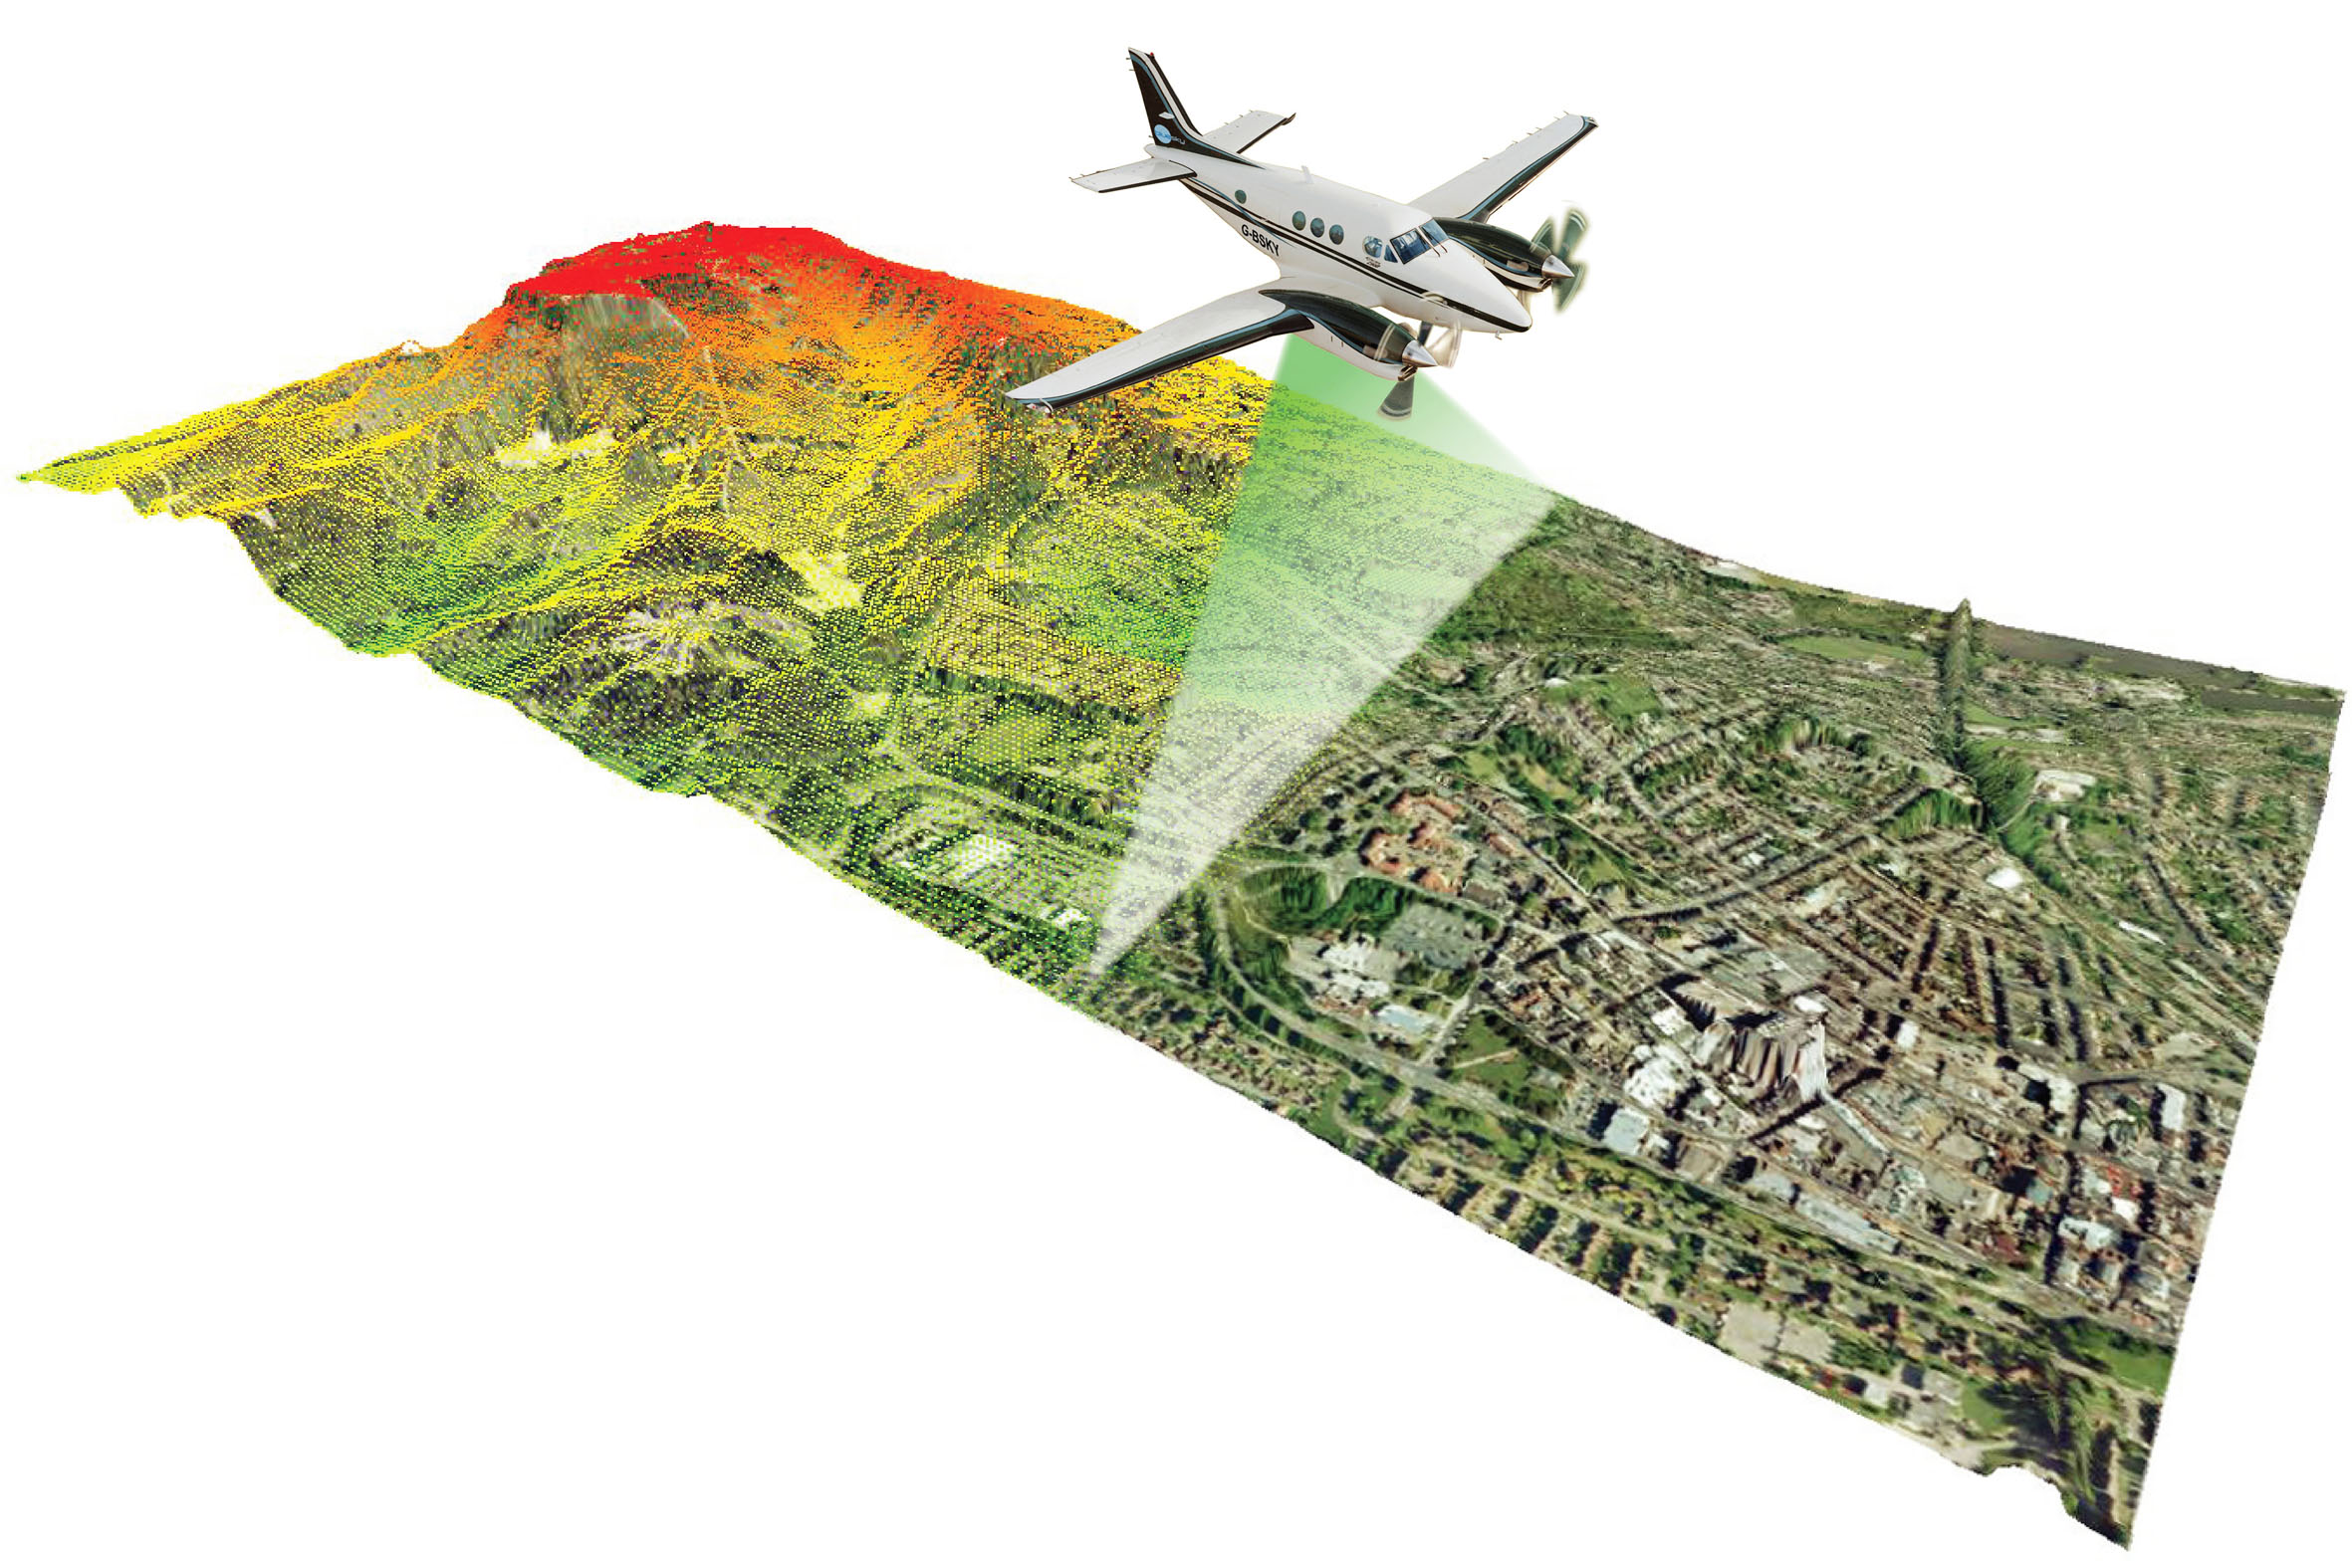
\includegraphics[width=1\textwidth]{img/LIDAR.jpg}
\caption{Schematycznie przedstawiony nalot podczas zbierania danych LIDAR}
\label{fig:lidar}
\end{figure}

Na rysunku \ref{fig:lidar} przedstawiono w sposób schematyczny jak przebiega pobieranie danych. Samolot podczas nalotu pobiera dane wzdłuż pewnego odcinka prostopadłego do kierunku lotu, z których następnie powstaje chmura punktów, której wizualizację również przedstawiono na rysunku.

\section{Opis wybranych algorytmów}

W poniższym rozdziale zostaną opisane istniejące algorytmy przetwarzania danych w postaci chmury punktów w systemach GIS.

\subsection{Triangulacja Delaunay'a}

\subsubsection{Definicja}
Triangulacja Delaunay'a jest reprezentacją chmury punktów w postaci nieregularnej siatki trójkątów TIN (z ang. Triangulated Irregular Network).
Jej cechą szczególną jest fakt, iż żaden z punktów nie leży wewnątrz okręgu opisanego na dowolnym trójkącie \cite{Lee1980}. Podział ten ma tę własność, że maksymalizuje najmniejszy kąt spośród 
wszystkich trójkątów należących do triangulacji. Na rysunku \ref{fig:triangulacja} przedstawiono przykładową triangulacje.

\begin{figure}[h!]
    \centering
    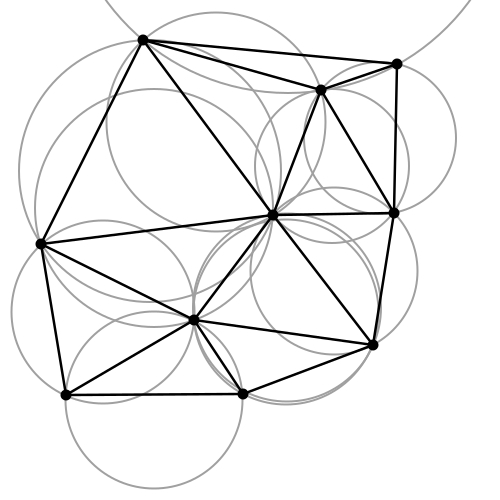
\includegraphics[width=0.5\textwidth]{img/triangulacja.jpg}
    \caption{Triangulacja Delaunay z zaznaczonymi okręgami opisanymi na trójkątach}
    \label{fig:triangulacja}
\end{figure}

\subsubsection{Aplikacje}
Triangulacja Delaunay'a jest często wykorzystywana przy przetwarzaniu danych LIDAR. Dzięki stosowaniu filtracji może służyć do oddzielania poszczególnych zbiorów punktów od siebie \cite{koziol2007} bądź też do znajdywania łamanej otaczającej zadany zbiór punktów \cite{website:HumanGeoBlog}. Istnieje wiele implementacji algorytmu pozwalającego na przetworzenie chmury punktów do postaci siatki trójkątów \cite{Lee1980,Dwyer1987,jiang2010}. W artykule \cite{Lee1980} opisano dwa algorytmy tworzenia takiej siatki - dziel i zwyciężaj oraz tribuild. Pierwszy z nich o złożoności obliczeniowej $O(N log N)$ rekurencyjnie dzieli zbiór punktów pośrednich na mniejsze zbiory, w nich dokonuje triangulacji a następnie łączy je. Drugi z nich o złożoności obliczeniowej $O(N^{3/2})$ zakłada znajomość prostokąta który otacza zadany zbiór punktów. Prostokąt ten jest dzielony na mniejsze, a następnie dla każdego mniejszego prostokąta:

\begin{algorithmic}
    \For {punkt P w punktach należących do prostokąta}
    \If {P jedyny punkt w prostokącie}
        \State połącz punkt z wierzchołkami prostokąta
    \Else
        \State dodaj krawędzie, aby nie zniszczyć triangulacji
    \EndIf
    \EndFor
\end{algorithmic}

Przykładowe kolejne etapy tak przeprowadzonej triangulacji pokazano na rysunku \ref{fig:iter_triangulacja}.

\begin{figure}[h!]
    \centering
    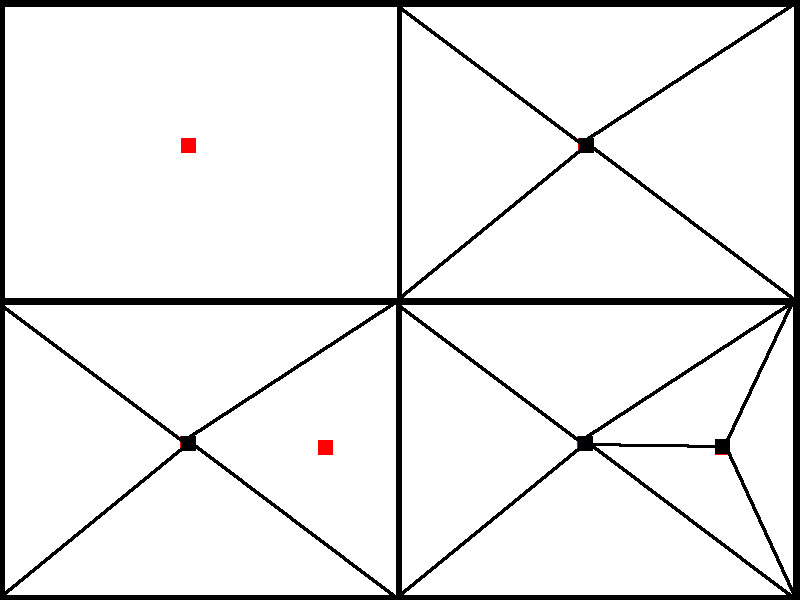
\includegraphics[width=0.5\textwidth]{img/iter_triangulacja.jpg}
    \caption{Iteracyjna triangulacja}
    \label{fig:iter_triangulacja}
\end{figure}

W 1987 Dwayer zaproponował szybszy algorytm dziel i zwyciężaj, o zakładanej złożoności $O(N log log N)$, jednak w pesymistycznym przypadku dalej będzie to $O(N log N)$  \cite{Dwyer1987}. Powstały też nowsze algorytmy pozwalające na stworzenie triangulacji. W artykule \textsl{An efficient algorithm for constructing Delaunay triangulation} autorzy zwracają uwagę, że w większości algorytmów szybko tworzy się siatkę a następnie dużo czasu poświęca się na lokalne optymalizacje, co skutkuje zwiększoną złożonością obliczeniową. Dzięki zaproponowaniu reguły prawej dłoni, udało im się znacząco zmniejszyć ilość obliczeń potrzebnych do przeprowadzenia lokalnych optymalizacji, tym samym proponowany algorytm ma złożoność na poziomie $O(N)$ \cite{jiang2010}.

\subsection{Maszyny wektorów nośnych}

\subsubsection{Definicja} 

Maszyny wektorów nośnych SVN (z ang. \textit{support vector machine}) pozwalają na rozwiązanie tzw. problemu klasyfikacji. Definicja problemu brzmi następująco: dla pewnej przestrzeni $\Omega$ zawierającej wektory danych x, należące do dwóch klas
$\Omega = \{(x_{i}, c_{i}) | x_{i} \in R^p, c_{i} \in \{-1,1\}\}$
należy znaleźć klasyfikator który podzieli tę przestrzeń na dwa rozłączne obszary jak najlepiej odpowiadające klasom $\{-1, 1\}$ \cite{stefanowski2010}. Do rozdzielenia zbioru na dwa służy tzw. liniowa funkcja separująca (lub jej uogólnienie - hiperpłaszczyzna dla przypadków n-wymiarowych), która wyznacza podział przestrzeni na dwa podobszary.

\begin{figure}[h!]
    \begin{subfigure}[b]{0.33\textwidth}
        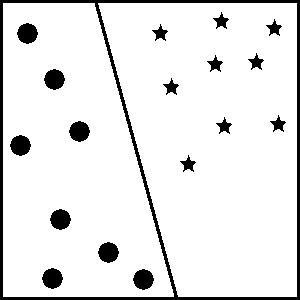
\includegraphics[width=\linewidth]{img/granica_1.jpg}
    \end{subfigure}%
    \begin{subfigure}[b]{0.33\textwidth}
        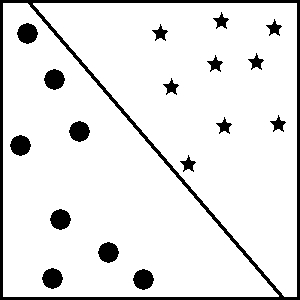
\includegraphics[width=\linewidth]{img/granica_2.jpg}
    \end{subfigure}%
    \begin{subfigure}[b]{0.33\textwidth}
        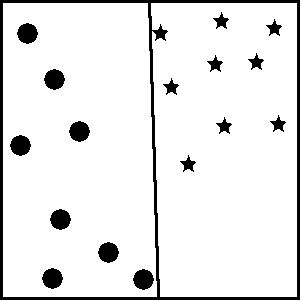
\includegraphics[width=\linewidth]{img/granica_3.jpg}
    \end{subfigure}
    \caption{Różne przykłady liniowej separacji}
    \label{fig:liniowa_separacja}
\end{figure}

Na rysunku \ref{fig:liniowa_separacja} przedstawiono różne poprawne sposoby separowania tego samego zbioru. Można w szczególności wyróżnić pary hiperpłaszczyzn $b_{i1}$ oraz $b_{i2}$, będących równoległych do 
siebie, powstałych poprzez przesuwanie jednej hiperpłaszczyzny od punktu granicznego pierwszego zbioru do punktu granicznego drugiego zbioru (rysunek \ref{fig:rownolegla_separacja}).

\begin{figure}[h!]
    \centering
    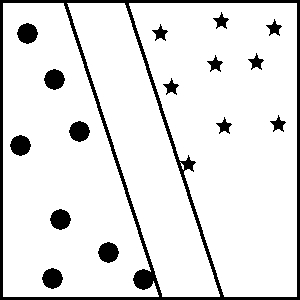
\includegraphics[width=0.33\textwidth]{img/granica_rownolegla.jpg}
    \caption{Równoległe hiperpłaszczyzny}
    \label{fig:rownolegla_separacja}
\end{figure}

Odległości pomiędzy hiperpłaszczyznami $b_{i1}$ oraz $b_{i2}$ nazywamy marginesem klasyfikatora liniowego. Maszyny wektorów nośnych znajdują taką hiperpłaszczyznę, która maksymalizuje margines. Szukamy więc hiperpłaszczyzny spełniającej warunki:

\begin{equation}
    w*x + b =0
\end{equation}

gdzie $w$ i $b$ są parametrami modelu. Wtedy przynależność do klas można wyrazić jako:

\begin{displaymath}
    y = \left\{ \begin{array}{ll}
        1 & \textrm{$w*x+b>0$}\\
        -1 & \textrm{$w*x+b<0$}\\
    \end{array} \right.
\end{displaymath}

Parametry $w$ i $b$ należy wyznaczać tak, aby maksymalne marginesy $b_{i1}$ i $b_{i2}$ były miejscem geometrycznym punktów $x$ spełniających warunki:
\begin{eqnarray}
    b_{i1} \quad w*x + b =1 \\
    b_{i2} \quad w*x + b =-1
\end{eqnarray}

\subsubsection{Aplikacje}

Możliowości wykorzystania maszyn wektorów nośnych do przetwarzania chmury punktów nasuwają się same - możliwe jest chociażby przydzielanie punktów do klas drzew i budynków \cite{xwang2011}. Istnieje wiele 
różnych przykładów na wykorzystanie SVN do przetwarzania chmur punktów \cite{xwang2011,li2013,david2015}. We wszystkich z nich część punktów pomiarowych jest wykorzystywana jako dane uczące.
Dla tych punktów operator ręcznie przydziela je do jednej z klas \cite{xwang2011}. Następnie na podstawie tych punktów możliwe jest określenie najlepszej hiperpłaszczyzny, jak opisano w sekcji \textit{definicja}.
W pracy z 2011r. wykorzystano tzw. niezbalansowane maszyny wektorów nośnych USVN (z ang. \textit{unbalanced support vector machines}) do rozróżnienia drzew i budynków \cite{xwang2011}.
Do analiz wykorzystano zdjęcia satelitarne oraz dane pochodzące z LIDARa - za pomocą tych dwóch źródeł stworzono wektory $x$ składające się z wysokości $Z$, wariancji wysokości $sZ$, różnice wysokości $hZ$,
pochodne 3-go rzędu wzdłuż osi X i Y - odpowiedno $dX$ i $dY$ - oraz wartość koloru RGB ze zdjęcia satelitarnego. 
W pracy \textit{Land classification from LiDAR full-waveforms based on multi-class support vector machines} wykorzystano SVM do przypisywania punktów do więcej niż dwóch klas \cite{li2013}. 
W innej pracy z 2015 równierz wykorzystano SVM do podziału zbioru na więcej niż dwie klasy \cite{david2015}. Analiza to posłużyła do zmierzenia powierzchni namorzyn na Filipinach. 
W tym przypadku do stworzenia wektorów $x$ wykorzystano numeryczny model powierzchmi DSM, numeryczny model terenu DTM, model wysokościowy CHM, średnią intensywność oraz ilość odbić. Co ciekawe, na podstawie
ilości odbić można określić gatunek drzewa \cite{Sasaki2012}.

\subsection{Analiza obrazu oparta obiektowo}

\subsubsection{Definicja}

Analiza obrazu oparta obiektowo OBIA (z ang. \textit{Object – based image analysis}) jest stosunkowo nową metodą \cite{burnett2003} służącą do przetwarzania obrazów. W przeciwieństwie do tradycyjnych metod przetwarzania, 
nie analizuje pojedynczych pikseli, lecz całe ich grupy, zwane obiektami. Ma to przypominać sposób, w jaki ludzie rozróżniają obiekty na zdjęciach. Jeżeli zdjęcia dotczą powierzchni ziemi (takie jak zdjęcia 
satelitarne) wyróżnia się wtedy metodę geograficznej analizy obrazu oparte obiektowo GEOBIA (z ang. \textit{Geographic Object-based Image Analysis}). Jako że tematyka całej pracy dotyczy systemów GIS,
w dalszej części będzie opisywana ten szczególny przypadek OBIA.

Metoda ta składa się z dwóch etapów. w Pierwszym z nich grupuje się podobne piksele (np. pod względem koloru) w obiekty prymitwne (prymitywy). Prymitywy służą następnie do konstruowania bardziej złożonych 
struktur, odpowiadających rzeczywistym obiektom takim jak jeziora czy drogi \cite{Blaschke2014}.  Budowanie obiektów może odbywać się stopniowo na poziome wielu wartstw, jak przedstawiono na rysunku
\ref{fig:poziomy_struktury}.

\begin{figure}[h!]
    \centering
    \includegraphics[width=0.5\textwidth]{img/obiekowa_analiza.png}
    \caption{Podział obrazu na piksele i obiekty}
    \label{fig:poziomy_struktury}
\end{figure}

\subsubsection{Aplikacje}
Metoda ta jest szeroko używana do analizy danych pochodzących ze skanowania laserowego. Jest wykorzystywana do klasyfikowania terenów miejskich \cite{zhou2013,chen2014},
wykrywania zmian powierzchni lasu \cite{zhang2014} oraz do wspomagania zarządzania terminalem kontenerowym \cite{tiede2015}. W tym ostatnim wykorzystano technikę OBIA do dokładnego określania miejsca położenia
kontenerów. Jest to zadanie o tyle łatwiejsze, iż wielkość kontenerów jest znana i podana jako norma ISO 668. Do celów analizy stworzono model DTM na podstawie danych LIDAR. Następnie do wykrywania
umiejscowie kontenerów wykorzystano dane LIDAR (pochodzące z jednego nalotu) oraz wykonywane częściej zdjęcia. Efektem jest model 3D nabrzeża.

Na polu analizy i klasyfikacji terenów miejskich metoda OBIA również odnosi sukcesy. Jednym z przykładów jest praca opisana w artkule z 2014 roku \cite{chen2014} w której autorzy za pomocą jedynie
danych LIDAR uzyskali dokładność klasfikacji punktów na poziomie  96.3\%. Wykorzystano w tym celu cztery informacje pochodzące ze skanowania - wysokość punktów nad poziomem gruntu, intensywność (czasem
nazywana amplitudą) oraz różnicę wysokości i intensywności pierwszego i ostatniego impulsu. Następnie podzielono obraz na prymitywy, jak opisano w sekcji Definicja. Na końcu nastąpiło przypisanie poszczególnych
obiektów do różnych klas na podstawie opisanych powyżej czterech atrybutów, jak przedstawia tabelka \ref{tab:przypisanie_do_klas}.

\begin{table}[h!]
    \centering
    \caption{Klasyfikacja terenów na podstawie cech}
    \label{tab:przypisanie_do_klas}
    \begin{tabular}{|c|c|c|c|}
        \hline
        Klasa & Wysokość & Intensywność & Różnica wysokości i intensywności\\
        \hline
        Trawniki & Niska & Wysoka & Bardzko niska\\
        \hline
        Trawa i roślinność & Niska & Średnia & Bardzo niska\\
        \hline
        Drogi i ziemia & Niska & Niska & Bardzo niska\\
        \hline
        Woda & Niska & Bliska 0 & Bardzo niska\\
        \hline
        Krzewy & Średnia & Średnia & Niska\\
        \hline
        Infrastruktura Publiczna & Średnia & Wysoka & Średnia\\
        \hline
        Drzewa & Duża & Wysoka & Duża\\
        \hline
        Budynki & Duża & Wysoka & Średnia\\
        \hline
    \end{tabular}
\end{table}

\section{Klasyfikacja danych}


\listoffigures
\addcontentsline{toc}{chapter}{Spis rysunków}
\listoftables
\addcontentsline{toc}{chapter}{Spis tabel}


\bibliographystyle{unsrt}
\bibliography{bibliografia}

%\begin{thebibliography}{20}
%\bibitem{Doktorat} K. Gunawickrama \textit{Leak detection methods}, Praca doktorska, Gdańsk, 2001.
%\end{thebibliography}

%*****************
%\begin{appendices}
%\chapter{Derivation of Pipe-flow Process Model}

Since the derivation of the model is based on physical relationships and conservation principles it would be convenient to study at least once the consecutive steps performed in order to obtain it. This may provide reader with better understanding of the process as well as present assumptions and approximations that are utilized. The model is derived starting from two equations: equation of continuity and equation of motion. The derivation provided below is based on \cite{billmann_isermann,keerthi_phd}.

\section{Equation of Continuity}

We start from definition of the mass:

\begin{equation}
\label{eq:mass}
m = \rho A \Delta z
\end{equation}

Considering mass change in time, i. e. mass-flow

\begin{equation}
\label{eq:massflow}
q = \frac{\partial m}{\partial t} = \rho A  w
\end{equation}

and then, introducing principle of conservation for elementary pipe segment we obtain

\begin{equation}
\label{eq:massflow2}
\frac{\partial m}{\partial t} = \rho A w - A\left(w + \frac{\partial w}{\partial z}\Delta z\right) \left( \rho + \frac{\partial \rho}{\partial z}\Delta z\right) 
\end{equation}

Substituting (\ref{eq:mass}) to  (\ref{eq:massflow2}) we obtain

\begin{equation}
\label{eq:massflow3}
\frac{\partial \left( \rho A \Delta z \right)}{\partial t} = \rho A  w - A\left( \rho w + \Delta z \left( \rho \frac{\partial w}{\partial z} +w \frac{\partial \rho}{\partial z} \right)+\frac{\partial w}{\partial z} \Delta z  \frac{\partial \rho}{\partial z} \Delta z  \right) 
\end{equation}

where the last term $\frac{\partial w}{\partial z} \Delta z  \frac{\partial \rho}{\partial z} \Delta z$ is small enough to be neglected. Then, substituting

\begin{equation}
\label{eq:ms4}
\rho \frac{\partial w}{\partial z} +w \frac{\partial \rho}{\partial z} = \frac{\partial}{\partial z} \left( \rho w \right)
\end{equation}

as

\begin{equation}
\label{eq:ms5}
\frac{\partial}{\partial z} \left( \rho w \right) + \frac{\partial \rho}{\partial t} = 0
\end{equation}

Assuming, that the process is isothermal we can introduce

\begin{equation}
\label{eq:ms6}
\nu = \sqrt{\frac{p}{\rho}}
\end{equation}

thus, substituting (\ref{eq:massflow}) and (\ref{eq:ms6}) to (\ref{eq:ms5}) we obtain first equation of our model:

\begin{equation}
\label{eq:cont_fin3}
\frac{A}{\nu^2} \frac{\partial p}{\partial t} + \frac{\partial q}{\partial z} = 0
\end{equation}


\section{Equation of Motion}

Here we start from definition of momentum:

\begin{equation}
\label{eq:mm1}
M = \rho A \Delta z w
\end{equation}

then,using principle of conservation:

\begin{equation}
\label{eq:mm2}
\frac{\partial \left( \rho A w \Delta z \right)}{\partial t} = A \left(p + \frac{\rho w^2}{2} \right) - A\left(p + \frac{\partial p}{\partial z} \Delta z + \frac{\rho w^2}{2} + \frac{\partial}{\partial z} \left( \frac{\rho w^2}{2} \right) \Delta z \right) - F - Y
\end{equation}

By rearranging equation presented above, we obtain:

\begin{equation}
\label{eq:mm3}
\frac{\partial \left( \rho A w \Delta z \right)}{\partial t} = A \left(p + \frac{\rho w^2}{2} \right) - A\left(\left(p + \frac{\rho w^2}{2} \right) + \Delta z \left( \frac{\partial p}{\partial z} +  \frac{\partial}{\partial z} \left( \frac{\rho w^2}{2} \right) \right)\right) - F - Y
\end{equation}

Substituting 

\begin{equation}
\label{eq:mm4}
 \frac{\partial}{\partial z} \left(p +  \frac{\rho w^2}{2} \right) = \frac{\partial p}{\partial z} +  \frac{\partial}{\partial z} \left( \frac{\rho w^2}{2} \right) 
\end{equation}

into (\ref{eq:mm3}) we will obtain
\begin{equation}
\label{eq:mm5}
\frac{\partial \left( \rho  w  \right)}{\partial t} = -  \frac{\partial}{\partial z} \left(p +  \frac{\rho w^2}{2} \right) - F- Y
\end{equation}

Again, assuming that the process is isothermal we obtain:

\begin{equation}
\label{eq:mm_fin}
\frac{1}{A} \frac{\partial q}{\partial t} + \left( 1 - \frac{q^2 \nu^2}{2 A^2 p}\right) \frac{\partial p}{\partial z} + \frac{q \nu^2}{A^2 p} \frac{\partial q}{\partial z}= - \frac{\lambda \nu^2}{2DA^2} \frac{q|q|}{p} - \frac{g sin \alpha}{\nu^2} p
\end{equation}

Taking into account, that if $w^2 \ll \nu^2$, i. e. velocity of the fluid is significantly lower than velocity of the sound in this fluid, we may neglect term $ \frac{q^2 \nu^2}{2 A^2 p}$. Moreover, if the pipeline is long, then we may neglect term $ \frac{q \nu^2}{A^2 p}$. Thus, we obtain second equation that is included in physical, continuous time model:

\begin{equation}
\label{eq:momen_fin3}
\frac{1}{A} \frac{\partial q}{\partial t} + \frac{\partial p}{\partial z} = - \frac{\lambda \nu^2}{2DA^2} \frac{q|q|}{p} - \frac{g sin \alpha}{\nu^2} p
\end{equation}

%\chapter{CD-ROM Content and Application Structure}

CD-ROM contains $\mbox{MATLAB}^{\mbox{\textregistered}}$ .m files that were developed while working on this thesis. In the main directory there is .pdf file with electronic version of this work. In the folder "sourcecode" there are following files:

\begin{itemize}
\item \textbf{wyzn2.m, wyznacznik.m} - files that were used to check whether determinant of recombination matrix has been properly calculated.
\item \textbf{accuracy3.m} - file used for evaluating accuracy of compared methods.
\item \textbf{kka\_accuracy\_norm.m} - file used for comparison of norms of residual matrices.
\item \textbf{pipe\_simulator.m, sym\_rur\_di.m} - both files were used to model leak and then check the models if they are able to produce correct estimates of leak size and location. Former one needs latter to work properly.

\end{itemize}

\section{Programming Environment and Program Description}

As stated above, all programs are in the form of $\mbox{MATLAB}^{\mbox{\textregistered}}$ files and are intended to work with this environment. In first position listed above is program for given matrix computes its determinant. Latter two positions consists of more complex programs, where the inversion of matrix is conducted using methods introduced earlier, where the methods are described in chapter 3. The last position on the list is the core part of the thesis that helps to evaluate the validity of the models, thus it is described briefly in following section.

\section{Pipe Simulator Application}

In order to check, whether the models produces proper results, the results are compared with the ones given by the model described in \cite{keerthi_phd}. General scheme of application is presented on figure \ref{fig:appl_scheme}.

\begin{figure}[ht]
   \centering
   \includegraphics[scale=0.75]{img/ldi_prog_scheme3.png}
   \caption{Scheme of pipe simulator used to evaluate validity of obtained results.}
\label{fig:appl_scheme}
\end{figure}

Application consists of two main subprograms: pipe simulator and leak detection and isolation.

\subsection{Pipe Simulator Program}

First subprogram is based on description provided in chapter 4. First step is to initialize the the pipe based on provided in program initial conditions, leak parameters and physical specification. From the initial conditions the state space model is constructed as in (\ref{eq:stan_pref5}). After the initialization there is a phase of simulation, where the values of $\hat{Q}_{in}, \hat{Q}_{ex}, \hat{P}_{in}$ and $\hat{P}_{ex}$ are determined. The data produced by that subprogram is treated as input data for leak detection and isolation system.

\subsection{Leak Detection and Isolation}

Second subprogram uses the data generated by pipe simulator. At first, there is an initialization to obtain state space model of pipe flow process with the same parameters as in pipe simulator. Further, the inversion of matrices is conducted using two methods introduced in chapter 3. After inversion three models are constructed and simulated in order to obtain estimates of inlet and outlet signals. After determination of these signals, the residuals are generated and processed in order to obtain the parameters of the leak.

\section{Application Manual}

To use the program, please open file "pipe\_simulator.m" it using $\mbox{MATLAB}^{\mbox{\textregistered}}$ version 7.0 or later. To specify the parameters of the pipe, its physical parameters can be changed by editing lines 10 to 20, where $Nd$ is number of the segments, $L$ length of the pipe, $c$ velocity of the sound, $Tl$ time of the leak, $Tr$ rise time of the leak, $zl$ location of the leak and $ql$ size of the leak. All values should be given in basic SI unit. Also, there is a possibility to change the number of simulation steps in line 3. After specification of physical parameters, press F5 button to start the simulation. In the main window of the program there will be information after every 1000 steps. At the end of pipe simulator subprogram the leak detection and identification part will be executed. After the simulation, the leak estimates are displayed in the form of figures. Each figure is properly labeled.

%\end{appendices}
%*****************

\end{document}
